\chapter*{Proposition 9}
\label{prop:9}


\begin{figure*}[ht]
    \begin{center}
    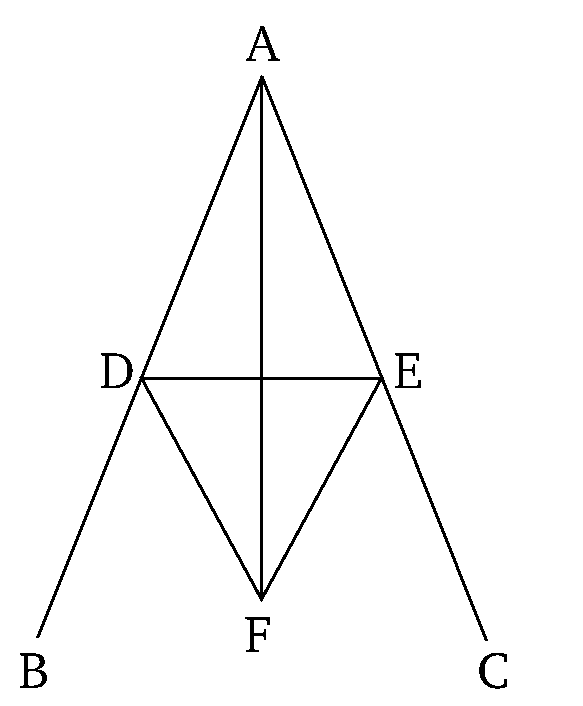
\includegraphics[width=0.5\linewidth]{figures/fig09e.eps}
    \label{fig:prop_9}
    \end{center}
\end{figure*}

To cut a given rectilinear angle in half.

Let $BAC$ be the given rectilinear angle. So it is required to
cut it in half.

Let the point $D$ have been taken at random on $AB$,
and let $AE$, equal to $AD$,  have been cut off from $AC$  [Prop.~1.3], and
let $DE$ have been joined. And let the equilateral triangle $DEF$
have been constructed upon $DE$ [Prop.~1.1], and let $AF$ have been
joined. I say that the angle $BAC$ has been cut in half by the straight-line
$AF$.

For since $AD$ is equal to  $AE$, and $AF$ is common, the two (straight-lines) $DA$,
$AF$ are equal to the two (straight-lines) $EA$, $AF$, respectively. And the base $DF$
is equal to the base $EF$. Thus, angle $DAF$ is equal to angle $EAF$ [Prop.~1.8].

Thus, the given rectilinear angle $BAC$ has been cut in half by the
straight-line $AF$. (Which is) the very thing it was required to do.


\section*{Commentary}

\begin{proposition}\label{proposition_9}\lean{Elements.Book1.proposition_9}\leanok
    Given an $\angle~BAC$, there must exist a point $F$, s.t., $F \neq A$ and $\angle~BAF = \angle~CAF$.
\end{proposition}
\begin{proof}
    \uses{proposition_1',proposition_3,proposition_5,proposition_5',proposition_7,proposition_8}\leanok
    Euclid's proof has two problems. First, when constructing $F$, it fails to state the requirement that $F$ and $A$ must be on different sides of $DE$.
    Second, Euclid did not rule out the possibility that $F$ lies on $AB$ or $AC$. If that could happen, 
    $\triangle~DAF$ or $\triangle~EAF$ wouldn't have existed, and the original proof would have failed.

    To prove $F$ is not on $AB$, let's first assume $F$ is on $AB$ (Fig.~\ref{fig:prop_9}). Apply Prop.~\ref{proposition_5} to $\triangle~ADE$ to derive $\angle~FDE = \angle~CED$. Apply Prop.~\ref{proposition_5'} to $\triangle~FDE$ to derive $\angle~FDE = \angle~FED$. Note that $\angle~CED~>~\angle~FED$. Contradiction.

    Similarly, we can prove $F$ is not on $AC$.
\end{proof}

\begin{figure*}[ht]
    \begin{center}
    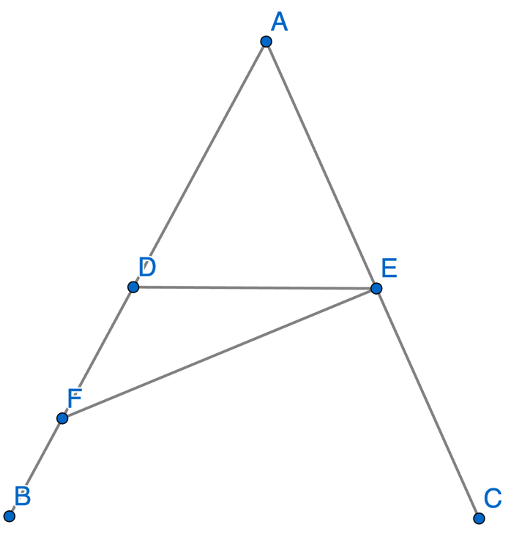
\includegraphics[width=0.5\linewidth]{figures/proposition_9.png}
    \label{fig:prop_9}
    \caption{$F$ on $AB$ cannot be true.}
    \end{center}
\end{figure*}

We can derive two additional properties of $F$: First, $F$ and $C$ must be on the same side of $AB$. Second, $F$ and $B$ must be on the same side of $AC$. 
Euclid did not include them in Prop.~\ref{proposition_9}, but they are necessary for later proofs.

\begin{proposition}\label{proposition_9'}\lean{Elements.Book1.proposition_9'}\leanok
    Given an $\angle~BAC$, there must exist a point $F$, s.t., $F \neq A$, $\angle~BAF = \angle~CAF$; $F$, $C$ are on the same side of $AB$; and $F$, $B$ are on the same side of $AC$.
\end{proposition}
\begin{proof}
    \uses{proposition_1',proposition_3,proposition_5,proposition_5',proposition_7,proposition_8}\leanok
    Same as the proof of Prop.~\ref{proposition_9}.
\end{proof}